\documentclass[conference]{IEEEtran}
\usepackage{blindtext}
\usepackage{graphicx}
\usepackage{amsmath}
\usepackage{algorithm,algpseudocode}


\makeatletter
\def\BState{\State\hskip-\ALG@thistlm}
\makeatother



\begin{document}
\title{Write an algorithm to round off a given decimal digit and plot the error/accuracy to
number of decimal digit for the solution of a quadratic equation.}

\author{\IEEEauthorblockN{Parag Parihar}
\IEEEauthorblockA{Roll No:- IIT2016095\\
iit2016095@iiita.ac.in}
\and
\IEEEauthorblockN{Rakshit Sai}
\IEEEauthorblockA{Roll No:- IIT2016126\\
iit2016126@iiita.ac.in}
\and
\IEEEauthorblockN{Adarsh Agrawal}
\IEEEauthorblockA{Roll No:- IIT2016516\\
iit2016516@iiita.ac.in}
\and
\IEEEauthorblockN{Nilotpal Pramanik}
\IEEEauthorblockA{Roll No:- IRM2016501\\
irm2016501@iiita.ac.in}
\thanks{Manuscript received February 2, 2018.}}

\markboth{Assignment-1, IDAA432C; B.Tech.(IT)}
{Shell \MakeLowercase{\textit{et al.}}: Bare Demo of IEEEtran.cls for Journals}

\maketitle

\IEEEpeerreviewmaketitle

\section{Introduction and Literature Survey}
The given task for us to design and analyze a problem. The given problem was to write an algorithm to round of a given decimal digit and plot the error or accuracy to number of decimal digit for the solution of quadratic equation. The given problem actually consists of two sets one is for rounding of the decimal digit and the other one is to calculate the roots and plot the error or accuracy graph.\\


According to the first problem, we have to round of a given decimal digit up to a certain digit.\\%for example let us take a number 139.59874 and let us say we have to round the given decimal number up to 3 digits, First we have to look at how many digits are there on the right side of the point and then if they are more than the given number of digits the decimal number has to be rounded of(Here 3) then the number itself is the answer and if it is more then(Here it is greater than 3) then we go on eliminating the digits starting from the rightmost digit. If the rightmost digit is less than 5 then we eliminate the rightmost digit and leave the digit just next to it unchanged, if the rightmost digit is more than 5 then we eliminate the rightmost digit and add 1 to the digit just next to it and if the rightmost digit is 5 then we see if the just next digit is even or odd, if even then we simply follow the steps given when the rightmost digit is greater than 5 and if it is odd then we simply follow the steps given when the rightmost digit is less than 5. So, by the given set of rules the answer for 139.59874 would be 139.599.%

In the second one we've to find the solutions of the quadratic equation. A quadratic equation of the form $ax^2+bx+c=0$ might have 2 distinct real solutions or 2 equal real solutions or 2 complex solutions.\\% It simply depends on the discriminant D which is $b^2-4ac$, if $D>0$ we get distinct real solutions, if $D=0$ we get 2 equal real solutions and if $D<0$ we get two complex solutions. %

After all this we need to draw a graph between error or accuracy and the number of digits of decimal number and check how much accurate the solutions we obtained are by rounding of them to a certain digit at each run and check the closeness of the quadratic equation to 0 when the root is substituted into it.\\

\section{Algorithm Design}
\textbf{An algorithm to round of a given decimal digit:-}\\

Firstly, we are going to take the input decimal number which is going to round of as an array of characters named “number”.As well as we are scanning the number up to which we have to round of the decimal number as the long int for all type of test cases.In “l” we have defined the length of the number as the input string.Also we have assigned 0 in the first index of an array of characters named “arr” to declare an extra digit at beginning.The purpose of the “arr” to store the whole digits (without point) from the decimal input.\\

Now we are traversing the “number” till it’s length defined in “l” to check at which index we are getting the point(.) assigned in “b”.If the input contains the point then that index will be stored in “point”, an int data type which already has been defined as “-1” by default.In other hand we’ll store other digits as characters in the “arr” array from the 1st index(arr[1]).\\

If point has “-1” value means the input is not containing any decimal point then we will check under this condition that if the length is equal to the “digit” then we’ll print the number given to us as input directly.Otherwise if the “digit” is less than the number then simply we’ll print “INVALID”,as it will be impossible.And where the digit is greater than the length we will print the number itself followed by the zeros of the difference between the digit and the length.\\

Where point is not “-1” means the input “number” containing the decimal point,and it is containing its location,we’ll check if the length of the numbers without the decimal point (through i-1) is equal to the “digit” or not.If true then we’ll similarly print the number itself and where the digit is greater than the length we will print the number itself followed by the zeros of the difference between the digit and the length.Then for the last case i.e where the digit is less than the length of the digits only firstly we have to check if the index of the decimal point i.e “point” contains greater value than the “digit” then we have to print “INVALID” again.Otherwise means where the digit is greater than the value at point  firstly we have to decrement the length and assign how many digits to be removed from the end of the number in x an int data type.\\

For while valid if the arr[i] contains value less than 5 we’ll put 0 in that position and otherwise if arr[i] contains value greater than 5 we are calling update function taking attributes as length, the total length to be removed from the end of the number and the array of size 2, containing the values respectively in the 0th and 1st indexes.In the “update function” till the the previous index of the particular index contains 9 the particular index will be filled as 0 and we’ll move to the beginning of the number by decrementing the length(i) and the value of x.Otherwise logically at that index 0 will be put and 1 will be added at the value of previous index.\\

Now if the value at the particular index is equal to 5 we will typecast it into int by subtracting  48 from it’s ASCII value and assign that at “value” and check weather it is even or not,If it is even to retain it’s value we’ll simply put 0 otherwise again call the “update” function to execute accordingly.\\

To proceed further we’ll decrement the value of length(i) and the value x accordingly and check weather the value of x is less than or equal to zero or not.If it is zero then we’ll break the loop through “break”.\\

If the the extra digit at the beginning of the arr i.e arr[0] retains 0 suggest the first digit of the input is not 9 and then from the index 1 of arr upto “digit” we’ll print the characters of the digits by checking the index of the point(“.”) to print it accordingly.Otherwise we’ll print digits similarly as previous way expect starting from the 0th index as the starting digit of the given input is 9.As well as we’ll check weather the index of the decimal point at “point” +1 ,i.e next index to the “point” is exceeding over the value of digit or not if true then it will print “INVALID” as through updating the decimal input finally the length of the number before the decimal point will be increased by 1 so logically having smaller “digit” to round of the input number will be impossible.
%\textbf{The error/accuracy to number of decimal digit for the solution of a quadratic equation.:-}
%Here we’ll take the coefficients of a quadratic equation as the inputs(a,b,c respectively) and assign the value of $b^2 - 4ac$ in d.If the value of d is greater than or equal to zero then we’ll assign the value of $\frac{-b + \sqrt{d}}{(2*a)}$ at root1 and  $\frac{-b - \sqrt{d}}{(2*a)}$ at root2.The both of the roots will be real.In other hand where d is less than zero we’ll print $\frac{-b}{2a}$ as the real part and  $\frac{\sqrt{-d}}{2a}$ as the imaginary part of the root1 similarly $\frac{-b}{2a}$ as the real part and $\frac{\sqrt{-d}}{2a}$ as the imaginary part of the root2.Here both the roots are imaginary.%
\begin{algorithm}[H]
\begin{algorithmic}[1]
\caption{update function}
\State \textbf{INPUT:-} i,x,a
\While{$arr[i] = '9'$}
    \State $arr[i] \gets '0'$
    \State $i \gets i-1, x \gets x-1$
\EndWhile
\State $arr[i] \gets '0'$
\State $arr[i-1] \gets arr[i-1]+1$
\State $a[0] \gets i, a[1] \gets x$
\end{algorithmic}
\end{algorithm}
\begin{algorithm}[H]
\caption{Rounding off any given number up to some significant digit}
\end{algorithm}
\begin{algorithmic}[1]
\State \textbf{INPUT: \textit{number}, \textit{sigdigit}}
\State \textbf{OUTPUT: Rounded off number}
\State \textbf{Initialization} :
\State $\textit{j} \gets 1, l \gets \text{length of }\textit{number}, \textit{arr[0]} \gets 0,i \gets 0$
\State copy \textit{\textbf{number}} into an character array \textit{\textbf{arr}} without "." and store the index of "." in \textit{\textbf{point}}
\If{ $\textit{point} = -1$}
    \If{ $length of number = \textit{sigdigit}$}
        \Return \textit{number}
    \ElsIf{ $length of number > \textit{sigdigit} $}
        \Return \text{invalid}
    \Else
        \State \text{print "\textit{number}."}
        \State add "rest zeroes"
    \EndIf
\Else
    \If{($length of number(excluding ".") = sigdigit$)}
        \State \text{print \textit{number}}
    \ElsIf{($length of number(excluding ".")< sigdigit$)}
        \State \text{print \textit{number}}
        \State add "rest zeroes"
    \Else
        \If{($point > sigdigit$)}
            \Return \text{invalid}
        \Else
            \State $i \gets i-1 , x \gets (i-point)-(sigdigit-point)$
            \While{($1$)}
                \If{($arr[i] < '5'$)}
                    \State $arr[i] \gets '0'$
                \ElsIf{($arr[i] > '5'$)}
                    \State $update(i,x,a)$
                \Else
                    \State $\textit{value} \gets arr[i-1] - 48$
                    \State if \textbf{value} is even update \textbf{arr[i] to  0} otherwise call \textbf{update(i,x,a)}
                \EndIf
                \State $ i \gets i-1, x \gets x-1$
                \If{$x <= 0$}
                    \State \textbf{break}
                \EndIf
            \EndWhile
        \EndIf
        \If{($arr[0] = 0$)}
            \State $i \gets 1$
            \While{($i <= sigdigit$)}
                \If{$i = point$}
                    \State \text{print "."}
                \EndIf
                \State \text{print $arr[i]$}
            \EndWhile
        \Else
            \If{$point+1 > sigdigit $}
                \State \text{print Invalid}
            \Else
                \State print the \textbf{arr} upto \textbf{sigdigit} with "."
            \EndIf
        \EndIf
    \EndIf
\EndIf

\end{algorithmic}



\textbf{The error/accuracy to number of decimal digit for the solution of a quadratic equation.:-}\\
Here we’ll take the coefficients of a quadratic equation as the inputs(a,b,c respectively) and assign the value of $b^2 - 4ac$ in d.If the value of d is greater than or equal to zero then we’ll assign the value of $\frac{-b + \sqrt{d}}{(2*a)}$ at root1 and  $\frac{-b - \sqrt{d}}{(2*a)}$ at root2.The both of the roots will be real.In other hand where d is less than zero we’ll print $\frac{-b}{2a}$ as the real part and  $\frac{\sqrt{-d}}{2a}$ as the imaginary part of the root1 similarly $\frac{-b}{2a}$ as the real part and $\frac{\sqrt{-d}}{2a}$ as the imaginary part of the root2.Here both the roots are imaginary.
\begin{algorithm}[H]
\begin{algorithmic}
\caption{Algorithm for finding root of given quardratic equation}
\State \textbf{INPUT:-} a,b,c
\State \textbf{OUTPUT:-} root1,root2
\State $d \gets b^2-4ac$
\If{$d>=0$}
    \State $root1 \gets \frac{(-b+\sqrt{d})}{2*a}$
    \State $root2 \gets \frac{(-b-\sqrt{d})}{2*a}$
\Else
    \State $root1 \gets \frac{-b}{2*a} + \frac{\sqrt{d}}{2*a}j$\\
    \State $root2 \gets \frac{-b}{2*a} - \frac{\sqrt{d}}{2*a}j$
\EndIf
\end{algorithmic}
\end{algorithm}
\section{Analysis and Discussion}
\subsection{For Algorithm:- 2}
\subsubsection{\textbf{BEST CASE-}}
\textit{The number of units of time taken for the FOR LOOP is:- $8n+2$
\\ $$time_{for\_loop} \propto 8n+2$$
\\ Total time is :-$8n+18$
\\\\\ $$time_{best\_case} \propto 8n+18$$}
 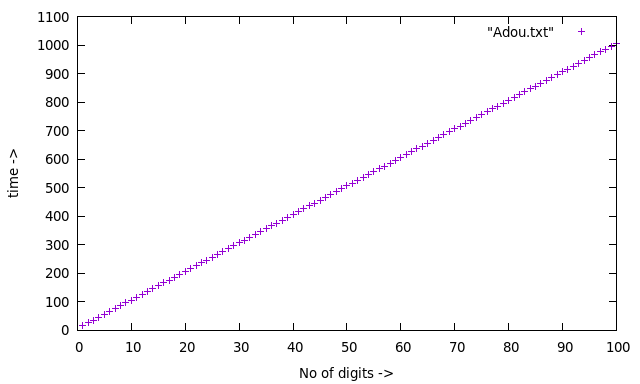
\includegraphics[height =  6.00cm,width = \linewidth]{bestcase_png.png}
\subsubsection{\textbf{WORST CASE-}}
The number of units of time taken for the FOR LOOP is:- $8n+3$
\\ $$time_{for\_loop} \propto 8n+3$$
\\The update function takes $9n+12$ units of time
\\\\ $$time_{update\_function} \propto 9n+12$$
\\The WHILE LOOP takes $(n-s)[9n+30]$ units of time
\\\\ $$time_{while\_loop} \propto (n-s)[9n+30]$$
\\ Total time is :-$9n^2 + 13n -9ns - 16s +7$
\\$$time_{worst\_case} \propto 9n^2 + 13n -9ns - 16s +7$$
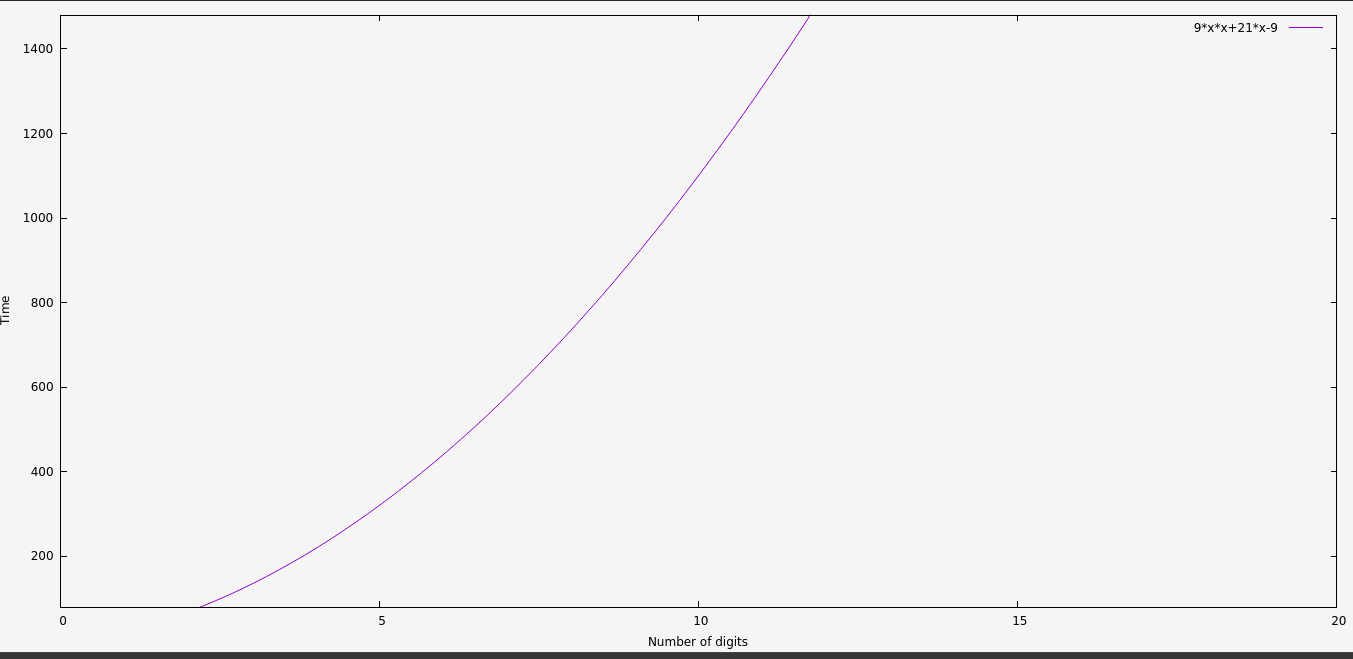
\includegraphics[height =  6.00cm,width = \linewidth]{worstcase.png}
\subsubsection{\textbf{AVERAGE CASE-}}
\textit{The number of units of time taken for the FOR LOOP is:- $8n+3$
\\ $$time_{for\_loop} \propto 8n+3$$
\\The number of units of time taken for the WHILE LOOP is:- $(n-s)(9)$
\\ $$time_{while\_loop} \propto (n-s)(9)$$
\\ Total time is :-$17n-9s+27$
\\ $$time_{average\_case} \propto 17n-9s+27$$}
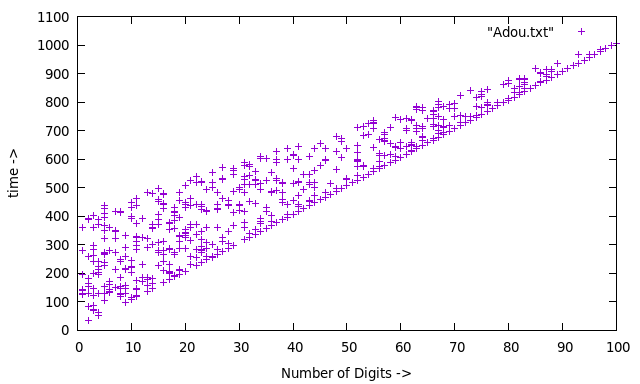
\includegraphics[height =  6.00cm,width = \linewidth]{averagecase_png.png}
\subsubsection{\textbf{Error/Accuracy Graph}}
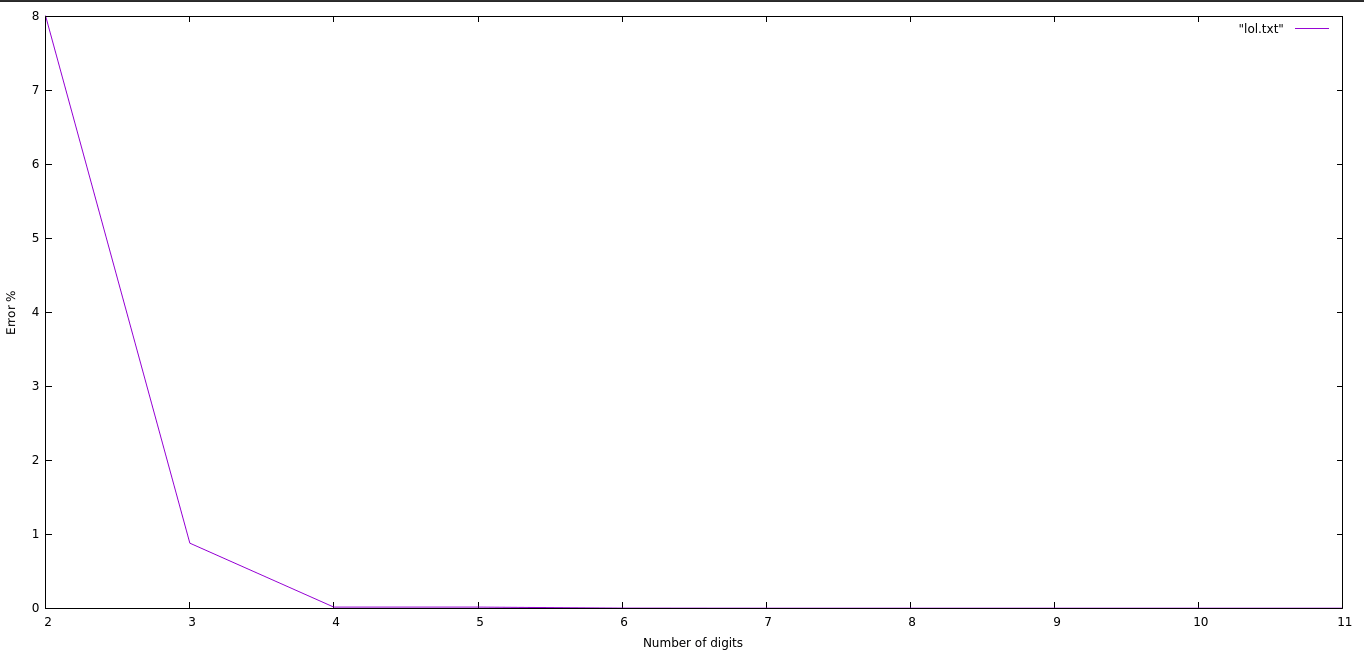
\includegraphics[height =  6.00cm,width = \linewidth]{errorex.png}

\subsection{For Algorithm:- 3}
In the case of \textbf{REAL ROOTS} we need 31 units of time and in the case of \textbf{IMAGINARY ROOTS} we need 29 units of time.
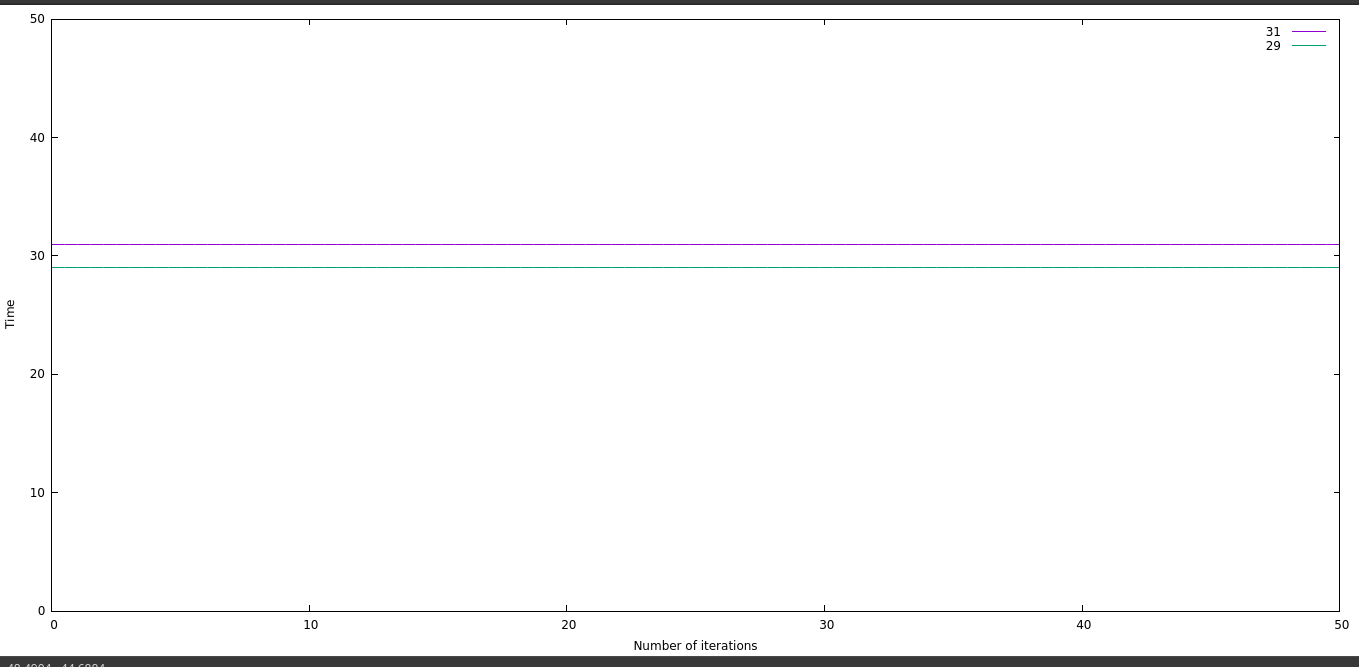
\includegraphics[height =  6.00cm,width = \linewidth]{quad2.png}
\section{Experimental Study}
\begin{table}[h!]
\begin{center}
    \caption{\textbf{PART A(For Algorithm 1)}}
    \label{tab:table1}
    \begin{tabular}{|l|c|r|} % <-- Alignments: 1st column left, 2nd middle and 3rd right, with vertical lines in between
    \hline
      \textbf{Initial decimal} & \textbf{Number of digits } & \textbf{Total instructions}\\
      \textbf{number} & \textbf{asked to round off} & \\
      \hline
      364 & 3 & 42\\
      \hline
      127345 & 6 & 66\\
      \hline
      143.465 & 9 & 81\\
      \hline
      135.1112 & 5 & 101\\
      \hline
	  134.56 & 3 & 146\\
      \hline
	  189.956 & 4 & 156\\
      \hline
	  999.9956 & 4& 223\\
      \hline
	  & Average  & 116\\
      \hline
    \end{tabular}
\end{center}
\end{table}
In the \textbf {first part}, we are going to round off a given decimal number to a specific number of digits.
Let us consider the example of 364 with rounding off  to 3 decimal digits.
Since the number has no decimal, so after copying through for loop, it will never take if condition and so the value of point will remain -1 and hence it will go to 1st if condition and check the length of number with digits required which is same and hence the output will be generated and hence it is best case with least instructions of 42, $\Omega(n)$.
But, on considering example 999.9956 and to round off to 4 decimal digits.
While copying the digits point will get a value of 3 as digits before point are 3, hence the first if condition will be false and in else part as the test case is not invalid it will go into the else part it will begin the rounding off of digits from the right end, but when it will come to 5(rounded off to 6), the 9 before it shall be incremented and made 0 and so all the followed 9s, but at the end the last 0(at arr[0]),it will become 1 and hence while printing also it will check the first condition and print 1000 as an output making it the worst case with 223 instruction $O(n^2)$. 
Considering any one average case like 135.1112 it has 101 instruction which is near to the average instructions we got of these 7 test cases.

\textbf {Graph Description :}

\textbf {Best Case :} Since there is only the first for loop running in that hence it is linear $O(n)$.
\textbf {Worst Case :} The worst case will have the for loop, the while loop will also include the while loop of ‘Update’ Function,which in this case case can run for n times and the above while will run for (n - required digits), hence it is of order $O(n^2)$ $\rightarrow$ $(n-s)*(n)$. 
\begin{table}[H]
\begin{center}
\caption{\textbf{PART B(For Algorithm 2)}}
	\label{tab:table2}
    \begin{tabular}{|l|r|}
    \hline
    \textbf{Quadratic Equations} & \textbf{Total instructions}\\
    \hline
    a = 1, b = -7, c = 12 & 31\\
    \hline
    a = 4, b = 1, c = 1 & 29 \\
	\hline
    a = 4, b = 4, c = 1 & 31\\
	\hline
    a = 7, b = 2, c = 2 & 29\\
	\hline
    \end{tabular}
\end{center}
\end{table}
In the \textbf{second part},% we are asked asked to plot the error accuracy graph of roots of quadratic equation, %
the time graph %are of order of $O(1)$, as it has loops, just checking of D, and hence it is “Theta” %
for this algorithm of order of $\theta(1)$.% as depicted in the graph.%
Consider any example, whether having complex or real roots, there will be some error in the roots of the quadratic equation, hence we are plotting error-accuracy against no of digits in the roots of the equation. %The more  digits in the root of the equation, hence we see an increase in accuracy but decrease in error with increase in number of digits. 
There will be an increasing in accuracy but decreasing graph in error with increase in number of digits. 

\section{Conclusion}
In the \textbf{first part} of the problem we have implemented it efficiently and try to analyze the algorithm correctly.By doing proper analysis of the code for rounding of the decimal number up to a given digit we found out that the time complexity for the worst case is proportional to $O (n^2)$ and the corresponding best case $\Omega(n)$.\\
In the \textbf{second part} of the problem throughout the analysis we can conclude that by increasing the digits the accuracy is increasing and error is decreasing because once we start rounding of the decimal roots of any quadratic equation the distance of the point from it's original value will be increased %that's why the accuracy will be increased accordingly.%
Therefore we get a exponentially decreasing graph and the  accuracy graph is exponentially increasing.As well as we found out that the time complexity for the worst case is proportional to $O(1)$ and the best case is $\Omega(1)$ same as the worst case hence, the time complexity will be $\Theta(1)$.

\end{document}
